\part{Experimental control}
\label{part:experiment}

\chapter{Experimental Testbed and Experiment Engines}%
\label{chapter:experiment:testbed}

    \section{State of the art}%
    \label{sec:state_of_the_art}

        \subsection{Grid'5000}%
        \label{sub:grid_5000}

            Nearly all the experiments presented in this document have been carried on the Grid'5000~\cite{grid5000}
            testbed.  Quoting its official website\footnote{\url{https://www.grid5000.fr/}}: \blockquote{Grid'5000 is a
            large-scale and flexible testbed for experiment-driven research in all areas of computer science, with a
            focus on parallel and distributed computing including Cloud, HPC and Big Data and AI.} It provides dozen of
            clusters, each one having between 2 and 124 homogeneous compute nodes. There is a high diversity of hardware,
            including several generations of Intel processors available, AMD and ARM processors, GPU, persistent memory
            (PMEM) as well as high-performance networks such as Infiniband or Omni-path. Another important feature is the
            ability for the experimenter to get full control on the nodes, as it is possible to deploy a new operating
            system and therefore to gain superuser access.

        \subsection{Experiment engines}%
        \label{sub:experiment_engines}

            While it is possible to run a complete experiment on a testbed like Grid'5000 by manually issuing commands
            in an interactive shell, it is not advisable as it quickly becomes extremly tedious and error-prone.
            Automating the experiment is a necessary condition to have reproducible results. A first step toward this
            goal is to write some ad-hoc script. However, two independent experiments might still share a lot of steps
            that could be refactored in a common layer, \eg OS deployment, package installation, or even more advanced
            features like node instrumentation or environment logging.

            For these reasons, it is a common practice to use an experiment engine. Buchert~\etal describe the features
            of eight different softwares~\cite{buchert:hal-01087519}. To the best of our knowledge, only three offer a
            native support for Grid'5000, namely Expo, XPFlow and Execo. Unfortunately, Expo and XPFlow are now longer
            maintained, the last commit in their respective repositories was done on November 2014 and September 2015
            For these reasons, the experiment engine Execo~\cite{Imbert_2013} is often recommended to Grid'5000
            newcomers.

            Experiments with Execo are described as a Python script. We believe this is one of its best qualities, as it
            offers a lot of freedom and flexibility to the experimenter, comparatively to other experiment engines that
            use custom domain specific languages (DSL). Yet, we made the choice to not use it. The main reason is that a
            typical Execo experiment uses a lot of low-level constructs that are really unpleasant and unintuitive to
            write and read. Section~\ref{sub:comparison_with_execo} will present some comparisons. Furthermore, Execo
            lacks a lot of important features, like node instrumentation and metadata collection, \ie we would still
            have needed to implement a lot functionnalities on top of Execo.

    \section{Yet another experiment engine: \texttt{peanut}}%
    \label{sec:peanut}
        %% TODO
        %% Différents moyens mis en oeuvre pour faciliter la reproductibilité (au sens
        %% large) :
        %% - Description structurée et lisible d'une expérience, relativement haut niveau
        %%   -> on comprend facilement ce qu'il se passe, on peut reproduire l'expérience
        %%   sans utiliser peanut.
        %% - Une fois l'expérience écrite, 100% automatisé, lancée avec juste une ligne de
        %%   commande.
        %% - Collecte d'information : commandes exécutées et leur std{out,err},
        %%   informations système, timestamps, monitoring.
        %% - Attention aux excès, pas forcément pertinent de collecter 10GB
        %%   d'info par expérience, voir même contre-productif si ça incite à ne
        %%   pas refaire les XP. Parler des problèmes découverts sur G5K (ref. au
        %%   dernier chapitre) ?
        %% - Future work: NIX & GUIX.
        %% - L'utilisateur garde le contrôle sur le plan d'expérience, grâce à des fichiers
        %%   d'expériences (peanut n'est pas chargé de randomiser l'xp). Ref à la prochaine
        %%   section.
        \subsection{Key features}%
        \label{sub:key_features}
            We implemented our own experiment engine, named \texttt{peanut}. It comes as a Python library that
            experimenters can use to write their own experiments, also as a Python script.

            A new experiment can be defined by inheriting from the class \texttt{peanut.Job}. Three methods can be
            overriden, \texttt{setup}, \texttt{run\_exp} and \texttt{teardown}.

            Once the experiment is written, it can be launched in a single command line. The following steps will
            happen.
            \begin{itemize}
                \item Implicitely, submit a job with the given characteristics (\eg cluster, number of nodes, walltime,
                    etc), then deploy the given OS image.
                \item Implicitely (but optionnaly) enable or disable some performance functionnalities like
                    hyperthreading, turboboost, C-states.
                \item Implicitely (but optionnaly) instrument the nodes to collect at a regular interval some system
                    metrics (\eg core frequencies and temperatures, CPU power consumption, network traffic, memory
                    consumption).
                \item Implicitely (but optionnaly) run the \texttt{stress} command on all the nodes to warm them up.
                \item Run the methods \texttt{setup}, \texttt{run\_exp} and \texttt{teardown} in that order.
                \item Produce a \texttt{zip} archive containing relevant results and metadata. The experimenter can
                    explicitely add any file to the archive. In addition, the following content is also implicitely
                    archived:
                    \begin{itemize}
                        \item Metrics collected with the aforementioned instrumentation.
                        \item Human-readable log of the commands issued during the experiment.
                        \item Machine-parsable log of the commands (in JSON format) with their timestamps and output
                            (both \texttt{stdin} and \texttt{stderr}).
                        \item Machine-parsable file (in Yaml format) containing relevant information like
                            the exact versions used for \texttt{peanut}, \texttt{gcc}, \texttt{MPI} and the Linux
                            kernel, the command line that was used to launch this experiment, the cluster and the list
                            of nodes, start and end timestamps for each of the three main methods, the list of the git
                            repositories cloned during this experiment with their remote URL and the git hash of the
                            checkout.
                        \item For each node, the content of the file \texttt{/proc/cpuinfo} as well as the output of the
                            commands \texttt{env}, \texttt{lstopo}, \texttt{lspci}, \texttt{dmidecode},
                            \texttt{lsmod}, \texttt{dmesg}.
                    \end{itemize}
            \end{itemize}
            In addition, the experiment can be executed interactively in a Python terminal. All the implicit
            functionnalities described previously can also be explicitely called (\eg there are methods
            \texttt{disable\_hyperthreading}, \texttt{start\_monitoring} and \texttt{perform\_stress}).

            An experiment can be parametrized by two means:
            \begin{itemize}
                \item An install file. This is a Yaml file that can be used to describe how the setup phase should be
                    done. Typically, it can contain the desired version for different softwares like OpenBLAS or
                    OpenMPI, but also the duration of the warmup or the frequency of the monitoring.
                \item An experiment file. These can be of any kind. A typical use case is to provide a CSV file where
                    each line is a particular piece of the experiment (\eg an individual call to \texttt{dgemm} and the
                    columns represent the parameters for these experiments (\eg the sizes \texttt{M}, \texttt{N} and
                    \texttt{K} used by \texttt{dgemm}).
            \end{itemize}

        \subsection{Comparison with Execo}%
        \label{sub:comparison_with_execo}

            In this section, we use a small example to illustrate some differences between \texttt{peanut} and
            \texttt{execo}. The goal is to write an experiment that will take several nodes on a given Grid'5000
            cluster, compile the \texttt{CRoaring} library\footnote{\url{https://github.com/RoaringBitmap/CRoaring}} and
            run one of its benchmarks.

            \lstdefinestyle{custom_lst_style}{
             %   language=Matlab,
                numbers=left,
                stepnumber=1,
                numbersep=10pt,
                tabsize=4,
                showspaces=false,
                showstringspaces=false
            }
            \lstset{basicstyle=\scriptsize, style=custom_lst_style}

            First, Listing~\ref{lst:engine:execo} shows such an experiment using Execo. Run with: \verb#python script.py#\\

            \lstinputlisting[language={Python},label={lst:engine:execo},
                caption={Small experiment example Execo}]{
                img/experiment/engine/mweExeco.py
            }

            This script, albeit fairly small, is already difficult to read in some places. For instance, lines 11-12,
            one has to write a complex query as a string as follows:

            \verb#OarSubmission("{cluster in ('dahu')}/nodes=2,walltime=00:20:00")#

            It would be much more pleasant to write it as follows:

            \verb#OarSubmission(cluster="dahu", nodes=2, walltime="00:20:00")#

            Now, Listing~\ref{lst:engine:peanut_class} demonstrates how the same experiment can be rewritten using Peanut
            in a much more concise and readable way.

            Run with: \verb#peanut script.py run tocornebize --deploy debian9-x64-base \#\\
            \verb#    --cluster dahu --nbnodes 2 --walltime 00:20:00#

            \lstinputlisting[language=Python,label={lst:engine:peanut_class},
                caption={Small experiment example using Peanut}]{
                img/experiment/engine/mwePeanut.py
            }

            The script is not only twice shorter, it is also much more elegant. Furthermore, it accomplishes much more
            than Listing~\ref{lst:engine:execo}, as it produces a peanut archive with all the metadata related to the
            experiment.

\chapter{Randomizing matters!}%
\label{chapter:experiment:randomizing}
    %% TODO
    %% Calibration experiments: randomisation. pour quoi faire ?
    %% 1. éviter les biais (randomisation de l'espace de paramètres)
    %%    - certaines valeurs peuvent être particulières et on peut vouloir
    %%      au contraire biaiser vers ces valeurs
    %% 2. éviter les perturbations transientes
    %%    - montée en charge vs. régime stationnaire
    %%
    %% Plusieurs exemples à citer (ref aux présentations qu'on aurrait dû
    %% faire à XUG@Rennes et à JLESC@Bonnes).
    Suppose some researcher wants to evaluate the memory bandwidth of their laptop. A first way to answer this question
    could be to write a small program that allocates a buffer, then write some data on this buffer with the
    \texttt{memset} function while measuring the duration of this operation. The problem is that the time taken to make
    this memory write may not be representative, the following writes would very probably have different durations due
    to cache effects.  Therefore, it would be better to make several measures that should then be carefuly analyzed
    (maybe simply taking the average, or perhaps there are some \emph{outliers} that should be removed). However, by
    doing so we only measure the performance of a write for a given size. The effective bandwidth could be very
    different with a smaller or a larger buffer. The natural solution here is to repeat these sequences of measures for
    several sizes.

    A general advice shared by experimental scientists in such situations is to randomize the experiments. In general,
    this randomization should happen for:
    \begin{itemize}
        \item The parameter space (in this example, the set of sizes that are evaluated). The goal is to avoid bias, for
            instance sizes that are a power of two may lead to a different performance. Note that in some occasions, as
            this chapter will illustrate, it is desirable to bias the experiment towards some particular values.
        \item The experiment order (in this example, the order of the sizes). The rational here is to avoid temporal
            perturbations. In particular, there are often at least two phases, a load build up which converges toward a
            steady state. There can also be changes that happen once the steady state is reached, \eg caused by some
            external source. By randomizing the order of the experiments, it becomes much easier to recognize an
            eventual temporal perturbation simply by plotting the data.
    \end{itemize}

    In this chapter, we will discuss several lessons learned for conducting faithful experiments, most of the time the
    hard way.

    \section{Experimental setup}%
    \label{sec:experimental_setup}

        All the experiments presented in this chapter share a common setup. They have been repeated on several nodes and
        follow the same steps:
        \begin{enumerate}
            \item Deploy and install a fresh OS on the node.
            \item Run the \texttt{stress} command for 10 minutes to warm the node.
            \item Start a background process\footnote{\url{https://github.com/Ezibenroc/ratatouille}} to monitor the
                core frequencies and temperature every second.
            \item On each core, run a custom
                code\footnote{\url{https://github.com/Ezibenroc/platform-calibration/src/calibration}}
                to measure the durations of a given operation (either \texttt{dgemm} or several MPI functions, depending
                on the experiment).
        \end{enumerate}

        Unless specified otherwise, we used nodes from the Dahu cluster from
        Grid'5000\footnote{\url{https://www.grid5000.fr/w/Grenoble:Hardware}}. Each of these nodes has two Intel Xeon
        Gold 6130 CPU, which are 16 core CPU from the Skylake generation. They have a base frequency of
        \NSI{2.1}{\giga\hertz} and a turbo frequency of up to \NSI{3.7}{\giga\hertz}, but their turbo frequency is
        limited to \NSI{2.4}{\giga\hertz} when their 16 cores are active and in AVX2
        mode\footnote{\url{https://en.wikichip.org/wiki/intel/xeon\_gold/6130}}. We have used
        OpenBLAS\footnote{\url{https://github.com/xianyi/OpenBLAS}} version~0.3.1 and
        OpenMPI\footnote{\url{https://github.com/open-mpi/ompi}} version~2.0.2 compiled with GCC version~6.3.0 on a
        Debian~9 installation with kernel version~4.9.0.

    \section{Randomizing the sizes}%
    \label{sec:randomizing_sizes}
        %% TODO
        %% - Randomization de l'ordre des XPs HPL aussi mais pas de problème notable.
        %% - Les performances de MPI_Send,Recv dépendent de l'ordre du fichier d'expérience
        %%   (bon mélange des tailles ou non).
        %% - Les performances de dgemm dépendent de l'échantillonnage et de
        %%   l'échantillon (tests de non régression)
        %% - Les performances de dgemm dépendent de K (attendu), mais il y a un effet
        %%   mémoire (plus inattendu). Pour certains cas, souhaitable de calibrer à K
        %%   fixé. Dans ce cas là, isoler l'expérience du reste, ne pas essayer de mélanger
        %%   avec d'autres K.
        Some text\dots

    \section{Randomizing the data}%
    \label{sec:randomizing_data}
        %% TODO
        %% - Les performances de dgemm dépendent du contenu de la matrice (random ou
        %%   constant par exemple). Ça serait causé par des bit flips dans le CPU qui
        %%   engendre une plus grande consommation (réutiliser le rapport).
        The work presented in this section has been published as a technical report\cite{cornebize:bitflips}. The
        content of this section is therefore a near-verbatim copy of this report.

        This experiment comes, yet again, from an unfortunate phenomenon we stumbled upon when calibrating the platform
        for our simulations. Our predictions were wrong, so we investigated a bit and we noticed a significant mismatch
        between the durations measured with our calibration code and the durations observed in HPL. We found out that,
        the performance of the \texttt{dgemm} function depends on the content of the matrix, which was unexpected.

        \subsection{Randomization of the matrix initialization}
        \label{sub:randomization_matrix_initialization}
            The three matrices are allocated once at the start of the program as a buffer of size \(N^2\) with
            \(N=2,048\). Then, their content is initialized in three different ways, depending on the experiment:
            \begin{enumerate}
                \item All the elements of the matrices are equal to some constant. We have tested with three different
                    values: 0, 0.987 and 1.
                \item The elements of the matrices are made of an increasing sequence in the interval \([0, 1]\). More
                    precisely, \texttt{mat[i] = i/(N\textasciicircum{}2-1)} for i in \([0, N^2-1]\).
                \item Each element of the matrix is randomly and uniformly sampled in the interval \([0, 1]\).
            \end{enumerate}

        Figure~\ref{fig:exp:bit-flips:method-perf} shows the evolution of the dgemm durations during the experiment.
        A clear temporal patterns can be distinguished, the performance is oscillating.  Furthermore, several layers can
        be seen, the durations of \texttt{dgemm} are the highest when the matrices are initialized randomly and the
        lowest when they are initialized with a constant value. The sequential initialization is in between.

        \begin{figure}[htbp]
            \centering
            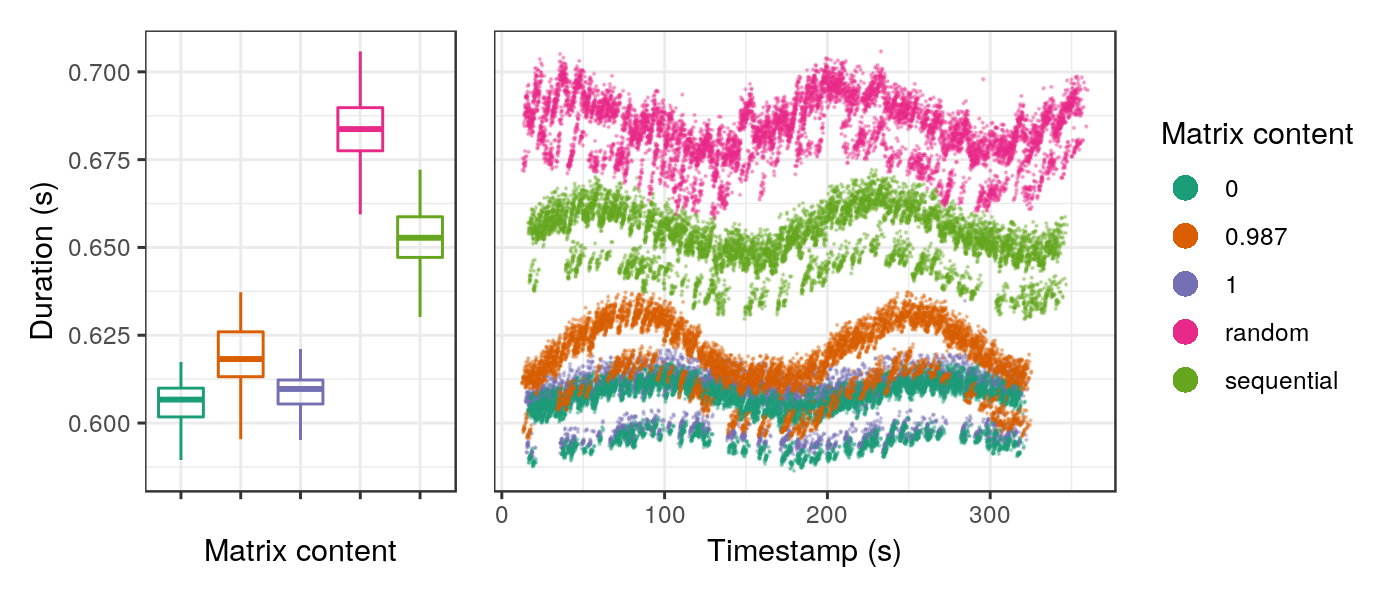
\includegraphics[width=\textwidth]{img/experiment/bit-flips/generation_method_perf.png}
            \caption{\label{fig:exp:bit-flips:method-perf}
            DGEMM durations are lower with constant values in the matrices}
        \end{figure}

        Such an observation was unforeseen. The function \texttt{dgemm} implements the usual matrix product with cubic
        complexity. The control flow of the function does not depend on the matrix content, so we did not expect its
        duration to be data-dependent.

        The observations we have made on \texttt{dgemm} performance can be explained by
        Figure~\ref{fig:exp:bit-flips:method-perf} which shows the evolution and the distribution of the core
        frequencies during the experiment. There is a clear correlation between the frequencies and \texttt{dgemm}
        performance: the random initialization produces lower frequencies whereas the constant initialization gives
        higher frequencies. A similar temporal patterns can also be distinguished with clear oscillations.

        \begin{figure}[htbp]
            \centering
            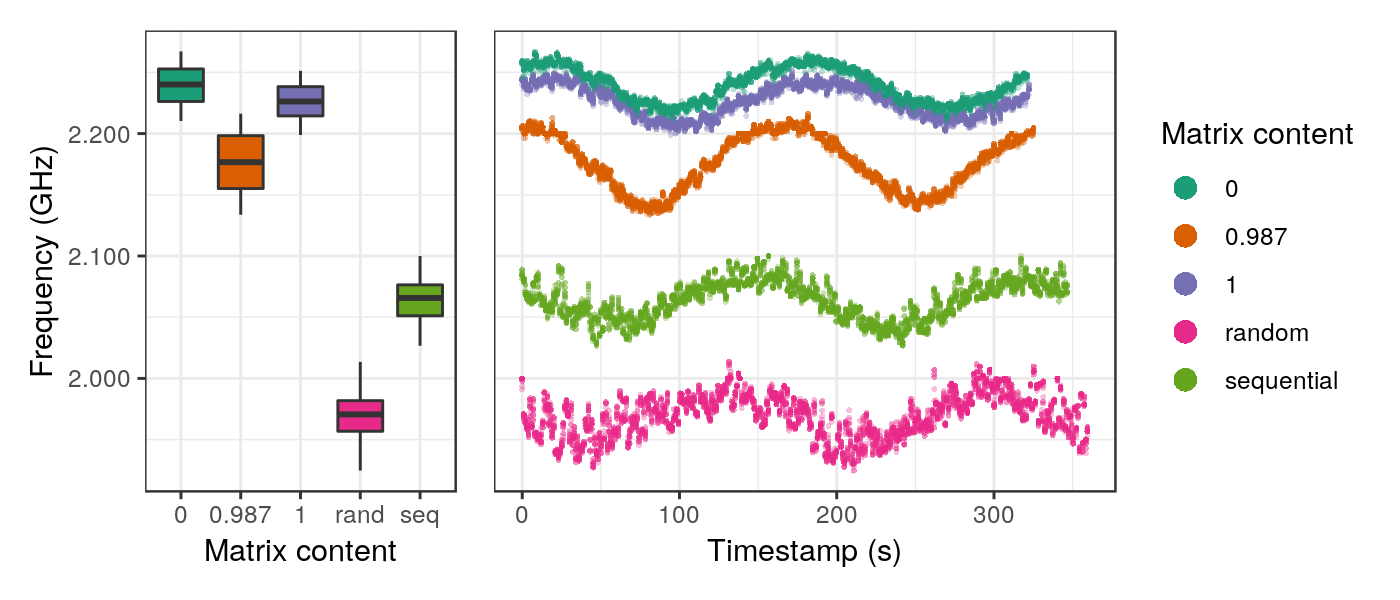
\includegraphics[width=0.9\textwidth]{img/experiment/bit-flips/generation_method_freq.png}
            \caption{\label{fig:exp:bit-flips:method-perf}
            Core frequencies are higher with constant values in the matrices}
        \end{figure}

        This experiment has been repeated on other Grid'5000 clusters, each time on at least four distinct nodes.
        Table~\ref{tab:bit-flips} gives a summary of our observations. Four other clusters show a similar behavior, the
        performance of \texttt{dgemm} is higher when the matrices are generated with a constant value. However, for four
        other clusters, this phenomenon could not be observed, the matrix content had no impact on the performance.
        %% TODO run this experiment on other Grid'5000 clusters, just to extend a bit the table of the clusters we tested it on.
        %% I have at least two clusters in mind:
        %% - pyxis (ARM processors)
        %% - troll (newest generation of Intel processors, Cascade Lake)

        \begin{table}[htbp]
            \caption{\label{tab:bit-flips}
            Observation of the  performance anomaly on Grid'5000 clusters}
            \centering
            \begin{tabular}{llll}
                \toprule
                Cluster & CPU & Generation & Performance anomaly\\
                \midrule
                dahu & Intel Xeon Gold 6130 & Skylake & yes\\
                yeti & Intel Xeon Gold 6130 & Skylake & yes\\
                ecotype & Intel Xeon E5-2630L v4 & Broadwell & yes\\
                gros & Intel Xeon Gold 5220 & Cascade Lake & yes\\
                parasilo & Intel Xeon E5-2630 v3 & Haswell & yes\\
                paranoia & Intel Xeon E5-2660 v2 & Ivy Bridge & no\\
                nova & Intel Xeon E5-2620 v4 & Broadwell & no\\
                taurus & Intel Xeon E5-2630 & Sandy Bridge & no\\
                chiclet & AMD EPYC 7301 & - & no\\
                \bottomrule
            \end{tabular}
        \end{table}

        \subsection{Hypotheses}
            %% TODO add the hypothesis on subnormal numbers.
            Several hypotheses were discussed to explain this unexpected phenomenon.

            There could be a small cache  on the floating point unit of the cores to memorize the results of frequent
            operations. This could explain why the durations were higher when the matrices were initialized randomly,
            but this does not explain why the sequential initialization is in between.

            This could be due to kernel same page merging (KSM), a mechanism that allows the kernel to share identical
            memory pages between different processes. Again, this would explain the difference between the random
            initialization and the constant one, but not why the sequential initialization gives intermediate
            performance.

            A last hypothesis is the power consumption of the cores. Each state change of the electronic gates of the
            CPU costs an energy overhead. In the case of the constant initialization, the registers will change less
            often during the execution of \texttt{dgemm}, in comparison with the random initialization. As for the
            sequential initialization, we can imagine that we have a locality effect: nearby elements of the matrices
            will have more bits in common, this would causes less bit flips than the random initialization but more bit
            flips than the constant initialization and thus an intermediate performance.



    \section{Beware of extrapolations}%
    \label{sec:beware_of_extrapolations}
        %% TODO
        %% Le problème est survenu dans plusieurs cas de figure, notamment
        %% pour HPL avec des géométries très élongées.
        %% - Les prédictions pour dgemm n'étaient plus très bonnes. On extrapolait trop
        %%   loin, la calibration était faite avec M<=15000 et N<=15000 alors que pour de
        %%   telles géométries on avait parfois des tailles 10\times plus grandes (les
        %%   produits MNK avaient le même ordre de grandeur par contre).
        %% - Les prédictions pour les communications étaient également mauvaises, en
        %%   partie parce que l'on calibrait pour des messages jusqu'à 1MB et on
        %%   esssayait de prédire la durée de communications de 1GB.
        Some text\dots

    \section{Beware of experimental conditions}%
    \label{sec:beware_of_experimental_conditions}
        %% TODO
		%% - Chauffe des CPU avant au cas où. Brice et Kevin monitoraient la
		%%   température au fil de l'expérience et arrêtaient les mesures quand
		%%   c'était trop chaud.
		%% - Dans HPL, il semble que les calculs ralentissent beaucoup certaines
		%%   communications. Ce phénomène n'était initialement pas capturé par la
		%%   calibration puisque les mesures étaient faites sans aucun calculs à
		%%   côté.
        Some text\dots

	\section{Conclusion}
		%% TODO
        %% - Certains facteurs extérieurs peuvent grandement impacter l'expérience, exemple
        %%   des problèmes de température sur dahu-{13,14,15,16}. D'où la nécessité de (1)
        %%   contrôler d'avantage l'environnement et (2) collecter d'avantage
        %%   d'informations sur l'environnement.
        Some text\dots


\chapter{Performance non-regression tests}%
\label{chapter:experiment:tests}
    %% TODO
    %% La partie précédente a montré que de nombreux problèmes peuvent survenir sur un
    %% testbed comme Grid'5000. Certains sont très visibles et vont être détectés
    %% rapidement (e.g. un disque HS), d'autres sont plus subtiles et peuvent passer
    %% inaperçu, faussant donc les expériences (e.g. performance inférieure de quelques
    %% pourcents). Dans cette partie, on essaye de détecter ces problèmes
    %% automatiquement.

    \section{State of the art}%
        %% TODO comment font les GAFAM ?
        Some text\dots

    \section{Performance measure and information collection}%
    \label{sec:performance_measure_and_information_collection}
        %% TODO
        %% Description du workflow mis en place, avec un joli dessin.
        %% - Génération du fichier d'expérience.
        %% - Soumission de jobs sur chaque cluster.
        %% - Réalisation de l'expérience, entièrement gérée par peanut.
        %% - Push automatique des résultats sur le dépôt gitlab.
        %% - Soumission d'un job CI pour extraire et agréger les informations des archives.
        %% - Réalisation des tests et courbes sur les données.
        Some text\dots

    \section{Statistical test}%
    \label{sec:statistical_test}
        Some text\dots
        %% TODO Reprendre le petit rapport que j'avais rédigé sur les stats derrières nos tests:
        %% /home/tom/Documents/Fac/phd/reports/2020/non_regression

    \section{Conclusion}%
    \label{sec:conclusion}
        %% TODO
        %% Raconter ce que l'on aurait pu faire et comment il faudrait l'étendre:
        %% - Test sur le modèle de dgemme plutôt que sur l'aggregated gflops
        %% - Test du modèle MPI (si on arrivait à définir et calculer les IC)
